\noindent
\textbf{On-chip Cache Architecture:} 
We propose \texttt{Elastic-Cache} to efficiently support both narrow and wide width data accesses from multiple memory locations to co-reside in a single cache line. 
We introduce a concept of chunk tags to store narrow width tags along with a conventional tag (dubbed commong tag) for each cache line (Figure~\ref{fig:elastic-cache}). 
This adds only a small area overhead, but allow us to efficiently use 128-byte cache lines for storing 16-, 32-, and 64-byte blocks from non-consecutive addresses, as well as a 128-byte block whose bytes are from consecutive addresses.
Figure~\ref{fig:elastic-cache-flow} describes the access flow of the proposed \texttt{Elastic-Cache}. 

\begin{wrapfigure}{r}[0pt]{0.4\textwidth}
\center
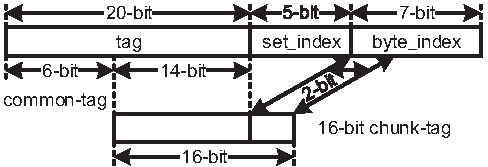
\includegraphics[width=1.0\linewidth]{./fig/chunk_tag_16bit-eps-converted-to.pdf}
\caption{The chunk and common tags to support both fine- and coarse-grained on-chip cache accesses for a 4-way 16KB cache.}
\label{fig:elastic-cache}
\end{wrapfigure}


To provide a cost-effective, large-capacity L2 cache, we will use eDRAM. 
Especially, to overcome relatively slow speed of eDRAM compared to SRAM, we propose a dynamic fine-grained spatial voltage boosting technique. 
In particular, this technique is beneficial for graph analytics that only need to access a small subset of a large eDRAM cache line without dissipating excessive power.

\begin{wrapfigure}{r}[0pt]{0.4\textwidth}
\center
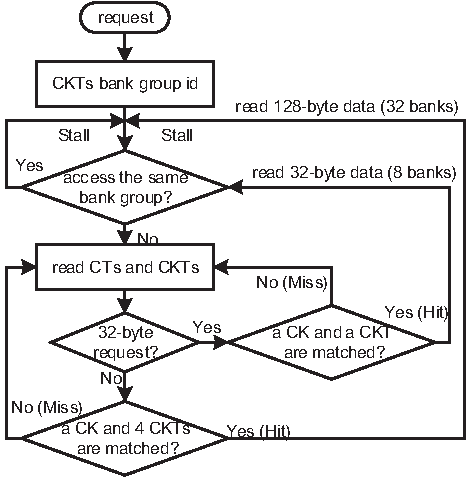
\includegraphics[width=1.0\linewidth]{./fig/flow_chart-eps-converted-to.pdf}
\caption{Access flow chart of chunk-tags and data. \texttt{CT}, \texttt{CKT}, and \texttt{CK} denote common tag, chunk tag, and chunk.}
\label{fig:elastic-cache-flow}
\end{wrapfigure}


Our proposed graph processor architecture needs both fine (4, 8, 16, 32 bytes) and coarse grained (64, 128 bytes) cache access. For the fine-grained access, it is sometimes preferable for cache systems to pack multiple data that are non-contiguous and not necessarily from the same row. These flexibilities can improve data movement patterns between main memory and cache in executing graph programs [HPCA’17]. 
Therefore, our goal in this part of project is to design eDRAM based cache to support such flexible access. Building upon our recent project to design ultra-low-leakage embedded SRAM design with temporal performance boosting capability [ISSCC’17], we will explore voltage boosting all the way to the thermal-limited level in a temporarily and spatially fine-grained fashion for improving access latency and throughput. For example, we can boost the supply voltage of the circuits that are involved in accessing a data of interest. We will also effectively gate or lower supply voltage of the circuits that are not involved in accessing the interested data, making them serving as thermal buffers. This way, we expect to significantly improve latency still under the thermal limit. In addition, by exploiting the latency improvement, we will explore to make the cache systems to perform multiple fine-grained data accesses (in serial by default but in parallel if data are in the multiple banks) and pack and send them back to the pipeline of a graph processor. 
To enable such voltage boosting, one of the key requirements is to stop voltage overdrive if temperature rises above a temperature limit. To do this, we need accurate thermal monitoring systems. Existing arts in on-chip thermal monitoring, however, have been limited due to sensor circuits that are too invasive in terms of size (> a few thousand µm2 per sensor) and voltage-scalability (requiring > 1V). This limitation prevents sensors from being placed closely to digital hotspots [ISSCC’12]. The resulted non-negligible distance between sensors and hotspots increases thermal monitoring error in the range of 10 to 20oC [TACO’08]. In this project, therefore we will create better thermal monitoring systems for eDRAM memory. We will build upon our recent sensor circuits [ISSCC’14, JSSC’15, CICC’15] that are very compact (30µm2/sensor) and voltage-scalable to share digital supply voltages. By placing such sensors closely to estimated hotspots, we can achieve high accuracy in thermal monitoring, which will allow us to use voltage boosting longer and more frequently without pessimistic throttling. Furthermore this will help a refreshing scheme to adaptively change refreshing periods, saving energy and increasing access availability in eDRAM. 


We will create circuit-level architectures to support temporarily and spatially fine-grained supply boosting to the thermal limited voltage level for shortening latency and increasing throughput. We will effectively gate or lower supply voltage of the circuits that are not involved in accessing a data of interest such that those circuits serves as thermal buffers. The gained throughput and latency improvement will be used to enable the flexible cache access to improve the performance of our proposed graph processor architecture. We will also create more accurate thermal monitoring systems to maximize the use of supply boosting without compromising robustness. Building upon our recent sensor circuits that are compact (30µm2/sensor) and voltage-scalable, we will place the sensors very closely to digital hotspots to improve thermal monitoring accuracy.
\noindent
\textbf{Off-chip Memory Architecture:} 
We aim to build our memory sub-system using Tezzaron’s DiRAM4 3D Memory for the main memory of our accelerator. 
One 8GB DiRAM die provides 64 32-bit ports (total 2048 I/O pins) with 1TB/s bandwidth. 
HBM2 is expected to provide the same bandwidth as DiRAM, but we choose DiRAM because DiRAM provides narrower but more memory channels (64×32-bit channels) than HBM2 (16×128-bit channels). 
That is DiRAM is more advantageous than HBM2 for graph analytics applications that generate random/irregular memory accesses. 
Especially, we will introduce a concept of dynamic memory channel formation where we dynamically group these 64 physical memory channels to form wider logical memory channels to efficiently service both random/irregular and sequential/regular memory accesses from the accelerators, depending on current memory access patterns. 
Subsequently, exploiting these many narrow memory channels, provided ``data-map,'' and relaxed synchronization, we will design an efficient memory controller with simple but large memory queues that allow us to coalesce as many random/irregular memory requests as possible.
